\documentclass[12pt,a4paper]{article}

\usepackage{styles/dolgozat}

\usepackage{listings}
% \usepackage{styles/cpp}
\usepackage{styles/python}
\usepackage{indentfirst}

\usepackage{hyperref}

\begin{document}

\pagestyle{empty} %a címlapon ne legyen semmi=empty, azaz nincs fejléc és lábléc

% A Miskolci Egyetem címere
{\large
\begin{center}
\vglue 1truecm
\textbf{\huge\textsc{Beszámoló szakmai gyakorlatról}}\\
\vglue 3truecm

\includegraphics[width=4.8truecm, height=4truecm]{images/me_logo.png}\\
\textbf{\textsc{Miskolci Egyetem}}
\end{center}}

\vglue 1.5truecm %függõleges helykihagyás

% A szakdolgozat címe, akár több sorban is
% A hallgató neve, évfolyam, szak(ok), a konzulens(ek) neve
{\large
\begin{center}
\begin{tabular}{c}
\textbf{Készítette:}\\
Hallgató Neve \\
Programtervező informatikus \\
Neptun kód: \texttt{N3P7UN} \\
e-mail cím: \texttt{e-mail@cim.hu}
\end{tabular}
\end{center}
\vskip 1cm
\begin{center}
\begin{tabular}{c}
\textbf{Üzemi instruktor:}\\
Piller Imre \\
tanársegéd \\
Alkalmazott Matematikai Intézeti Tanszék, Miskolci Egyetem \\
telefonszám: \texttt{+3646/565-111/14-50}


\end{tabular}
\end{center}}
\vfill
% Keltezés: Hely, év
{\large
\begin{center}
\textbf{\textsc{Miskolc, 2025}}
\end{center}}

\newpage


\newpage

\pagestyle{empty}

\cleardoublepage
\pagenumbering{gobble}
\tableofcontents
\cleardoublepage
\pagenumbering{arabic}

\newpage

\pagestyle{fancy}

\section{A feladat bemutatása}

A „Túlélés a Szocializmusban” című projekt egy különleges játékterv, amely a szocialista korszak mindennapjainak nehézségeit állítja a középpontba. Nem egy klasszikus akciójátékról vagy hősöket felvonultató történetről van szó, hanem egy olyan szimulációról, amely a túlélés, a döntéshozatal és a morális dilemmák kérdését vizsgálja. A játék lényege, hogy a játékos egy átlagember szemszögéből tapasztalja meg, milyen volt helytállni egy olyan rendszerben, ahol a választási lehetőségek gyakran szűkösek, a kockázatok pedig jelentősek. A projekt célja egyszerre a szórakoztatás és az elgondolkodtatás: miközben a játékos a túlélésért küzd, folyamatosan szembesül a korszak társadalmi és pszichológiai valóságával.

A célközönséget elsősorban azok a játékosok alkotják, akik értékelik a mélyebb tartalmat és a történelmi reflexiót. A játék azoknak szól, akik szeretik, ha döntéseik hosszú távon befolyásolják a játékmenetet, és nem riadnak vissza a morális dilemmáktól sem. Mivel a szocialista éra valós problémáit dolgozza fel, a játék különösen érdekes lehet történelemkedvelőknek, stratégiai játékok rajongóinak, de bárkinek, aki kíváncsi arra, hogyan éltek és túléltek emberek egy korlátozó társadalmi rendszerben. A felnőtt közönség számára ez nemcsak játék, hanem egyfajta interaktív társadalmi tükör is.

A mechanikai szinten a játék többféle munkalehetőséget kínál, például autószerelést, bolti munkát vagy irodai feladatokat. Ezek nemcsak eltérő játékmenetet biztosítanak, hanem más-más kihívásokat is hordoznak. A játékos állapotát különféle mutatók jelzik, mint az éhség, a stressz vagy a reputáció, amelyek egyensúlyban tartása folyamatos döntési kényszert eredményez. A rendszerbe beépített véletlenszerű események – például hatósági ellenőrzések vagy betegség – tovább erősítik a kiszámíthatatlanságot, így a játékosnak mindig újra kell terveznie stratégiáját. A morális dilemmák szintén hangsúlyosak: elvállaljon-e valaki kenőpénzes munkát, lopjon-e, ha családja éhezik, vagy vállalja inkább a nélkülözést?

A projekt különlegessége, hogy a megszokott nyugati kapitalista logikától eltérő játékkörnyezetet kínál. Kevés olyan játék született eddig, amely a szocializmus hétköznapi szintű tapasztalatait hitelesen mutatná be. Ez a játék képes arra, hogy a játékosokat belehelyezze egy olyan világba, ahol a mindennapi döntések komoly következményekkel járnak, és ahol a túlélés nem csupán anyagi, hanem lelki és erkölcsi kérdés is. A hitelességet tovább erősíti a gazdasági rendszer, amelyben a pénz mellett a cserekereskedelem és a feketepiac is szerepet kap.

Összességében a „Túlélés a Szocializmusban” nem csupán egy túlélő szimuláció, hanem egy interaktív történeti és társadalmi kísérlet. A játék egyszerre ad teret a stratégiai gondolkodásnak, az empátiának és a morális önvizsgálatnak. Ez a projekt azért különleges, mert képes a múlt egy darabját élményszerűen, de gondolatébresztő módon bemutatni, és ezzel egy hiánypótló szerepet betölteni a videójátékok világában.

\section{Technológia kiválasztása}

A projekt megvalósításához a Godot játékmotor került kiválasztásra, amely nyílt forráskódú, platformfüggetlen és alacsony rendszerigényű megoldást kínál \cite{godot_docs}. A motor előnye, hogy jól támogatja a 2D-s és kisebb volumenű 3D-s játékok fejlesztését, emellett a tanulási görbéje kedvező a kezdő fejlesztőcsapatok számára. 

A verziókövetéshez a GitHub szolgáltatása került kiválasztásra, amely biztosítja a kollaboratív fejlesztéshez szükséges átláthatóságot, a verziók nyomon követését és az esetleges hibák visszakereshetőségét.

A rendszer modularitásra épít, ami hosszú távon egyszerűsíti a bővítéseket és az új funkciók integrálását. A választott technológiák mindegyike hozzájárul a gyors prototípus-fejlesztéshez és az iteratív munkafolyamat támogatásához. Összességében a kiválasztott eszközök megfelelő egyensúlyt teremtenek a fejlesztési rugalmasság, a fenntarthatóság és a technikai stabilitás között, így biztosítva a projekt céljainak teljesíthetőségét.


\section{A tervezés folyamata}

A játék fejlesztésén összesen négyen dolgoztunk. Minden csapattag egyformán kivette a részét a projekt különböző részeinek megvalósításából. Dokumentálásban, programozásban és tesztelésben, grafikai részek elkészítésében kamatoztattuk a tudásunkat valamint új ismereteket szereztünk. Az elszántság és a rugalmas hozzáállás gördülékeny munkát eredményezett a csapatunk tagjai között.

Személy szerint a projekt tervezése során új ötletekkel valamint a dokumentálás létrejöttéhez szükséges utánajárással és ennek megvalósításával tudtam plusz segítséget adni a munkálatokhoz a fent említett feladatokon kívül.


\subsection{Előkészületek}

A projektünk elkészítése előtt fontos volt kineveznünk egy csapatvezetőt aki koordinálja a munkát és lehetővé teszi a a kommunikációt a gyakorlatvezetőnkkel. Ez nagy szerepet játszott abban is, hogy egyes feladatok felosztása, valamint ezek határidejének betartása probléma nélkül működjön.  Ezután tisztáztuk, hogy szükséges elkészítenünk egy vízió dokumentumot amely gyökeresen leírja a játék alapjait valamint, hogy miket szeretnénk pontosan elérni.
Ebből a dokumentumból az általam készített rész főbb pontjai:


\textbf{Felhasználói szerepkörök és projekt hatókör:}
\begin{itemize}
    \item Felhasználói szerepkörök ezen belül "Játékos", "Admin/Fejlesztő", "Vendég" céljainak leírása
    \item Projekt hatókör tartalmának leírása (pl: alap státuszok és mutatók), valamint ami kívül esik a hatókörön (pl: felhőalapú mentés)
\end{itemize}



\begin{table}[h!]
\centering
\caption{Időbeosztás és ütemezés a projektre vonatkozóan}
\label{tab:project_schedule}
\begin{tabular}{|c|p{4cm}|p{6cm}|c|c|}
\hline
\textbf{Hét} & \textbf{Tevékenység} & \textbf{Eredmény} & \textbf{Felelős(ök)} \\ \hline
1–2. & Dokumentáció & Vízió dokumentum, követelmények tisztázása & Teljes csapat \\ \hline
3–4. & Grafikai tervezés és modellezés & 2D háttérgrafikák, alap 3D modellek & Teljes csapat \\ \hline
5–6. & Programozás & Alap játékmenet és UI váz kialakítása & Teljes csapat \\ \hline
7. & Tesztelés, hibajavítás & Főbb hibák javítása, játékmenet stabilizálása & Teljes csapat  \\ \hline
8. & Véglegesítés & Projekt részleges lezárása & Teljes csapat \\ \hline
\end{tabular}
\end{table}

\subsection{Időbeosztás és ütemezés}

A projekt megvalósításához összesen nyolc hét állt rendelkezésünkre, amelyet kisebb szakaszokra osztottunk fel. Az első két hétben a dokumentáció elkészítése és a játék alapjainak lefektetése volt a fő feladat. A harmadik és negyedik hétre a grafikai elemek megtervezését és a 3D modellek létrehozását tűztük ki célul. Az ötödik és hatodik héten a programozásé volt a főszerep, amikor a játékmenet alapjait és a felhasználói felület vázát építettük fel. A hetedik hét főként a hibajavításról és a rendszer finomhangolásáról szólt. A nyolcadik hétre a véglegesítettük az eddig elkészült részeket.

A feladatokat úgy osztottuk be, hogy minden szakaszban mindenki aktív szerepet kapjon, de mindig volt egy felelős, aki az adott rész haladását koordinálta. Bár előfordult, hogy egy-egy rész feladatai átnyúltak a következő hétre, a rugalmas hozzáállásnak köszönhetően sikerült tartanunk az ütemtervet.

\subsection{Dokumentáció}
A projekt során segítettem a dokumentáció elkészítését. A kezdeti lépések között szerepelt a projekt felépítésének megtervezése, a fejlesztési ütemezés rögzítése, valamint a tájékoztató jellegű dokumentumok elkészítése és beépítése a projekttervbe. A vízió dokumentum tartalmi bontását közösen végeztük el. Az SRS dokumentumon belül én állítottam össze a „Megbízhatóság”, „Teljesítmény”, „Támogatottság” és „Tervezési korlátozások” részeket.

Az analízis modell elkészítésében is közreműködtem: részt vettem az osztálydiagramok, a különféle alrendszerek és a menürendszer felépítésének kidolgozásában. Például az "Interakciók és Karakter" Alrendszeren belül az "Interakciók alrendszer" felépítésének ábrázolásával járultam hozzá a munkálatokhoz. Az analízis modell elkészítése során diagramok jelentős részét a Visual Paradigm online szerkesztő segítségével hoztunk létre \cite{visual_paradigm}.

\begin{figure}[h]
    \centering
    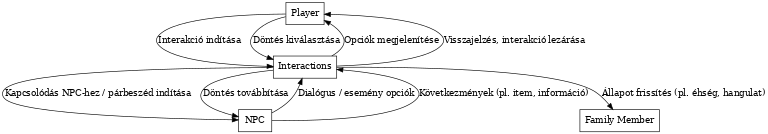
\includegraphics[width=0.9\textwidth]{latex/images/interactions_dynamic.png}
    \caption{Interakciók alrendszer}
    \label{fig:classdia}
\end{figure}

Emellett segítettem a grafikai elemek – például textúrák – hozzáadásában, illetve az általam elkészült részekben felmerülő hibák kijavításában. A dokumentációban a saját elemeim mindig naprakészek voltak a felmerülő változásokat követve.


\section{Implementáció}

A játék megvalósítása a Godot Engine keretrendszerben történt, amely jól támogatta a moduláris felépítést és a gyors prototípus-készítést. A projektben a jelenetek (scenes), a szkriptek és a grafikai elemek külön fájlokban kerültek kialakításra, így a csapattagok párhuzamosan tudtak dolgozni a saját moduljaikon. A verziókezelés biztosította a stabil integrációt, miközben a célunk egy játszható és stabil prototípus létrehozása volt, amely alapként szolgált a további fejlesztésekhez. A játékmechanikák moduláris kialakítása lehetővé tette az egyszerű bővíthetőséget és karbantarthatóságot \cite{godot_best_practices}.

\subsection{Felhasználói felület és HUD}

A játék során kiemelt szerepet kapott a felhasználói felület (UI) és a HUD (Head-Up Display) kialakítása. A cél az volt, hogy a játékos egyszerre kapjon visszajelzést a főbb állapotairól (éhség, stressz, alkoholszint, pénz), miközben az interfész ne terhelje túl a képernyőt.  
A HUD elemei külön jelenetként lettek létrehozva, és a fő játék jelenethez kapcsolódtak, ezáltal könnyen bővíthetővé váltak. A menük és visszajelző elemek egységes színvilágot kaptak, hogy illeszkedjenek a játék hangulatához.  

A megoldás előnye, hogy a HUD bármikor frissíthető a játékos aktuális állapotának megfelelően, és a játékmenet közben is reagál az eseményekre, például amikor a játékos pénzt keres vagy elveszít, illetve ha az éhség szintje megnő.


\subsection{Játékmechanikák implementálása}

A játék különböző mechanikáit modulárisan valósítottuk meg, így könnyen bővíthetők és
karbantarthatók maradtak. Egy ilyen mechanika például az inventory rendszer, amely a
játékos által gyűjtött tárgyakat és azok mennyiségét kezeli.

Az inventory megvalósítása lehetővé tette, hogy a játékos különféle tárgyakat gyűjtsön, kezeljen és felhasználjon a játékmenet során. A rendszer központi eleme egy szkript, amely egy szótárban (\texttt{Dictionary}) tartja nyilván az összes megszerzett tárgyat és azok mennyiségét. Ez biztosítja, hogy az inventory rugalmasan bővíthető legyen új tárgytípusokkal anélkül, hogy a teljes kódot át kellene alakítani.  


Az alábbi kódrészlet mutatja az inventory kezelésének fő funkcióit:  


\begin{python}
extends Node

var items : Dictionary = {}

func add_item(name: String, amount: int = 1):
	if not items.has(name):
		items[name] = 0
	items[name] += amount

func remove_item(name: String, amount: int = 1):
	if items.has(name):
		items[name] = max(0, items[name] - amount)
		if items[name] == 0:
			items.erase(name)

func has_item(name: String, amount: int = 1) -> bool:
	return items.has(name) and items[name] >= amount

func list_items() -> Dictionary:
	return items
\end{python}

A szkript négy fő funkciót lát el:  
\begin{itemize}
    \item \texttt{add\_item}: új tárgy hozzáadása az inventory-hoz, vagy a meglévő mennyiség növelése,  
    \item \texttt{remove\_item}: tárgy mennyiségének csökkentése, illetve törlése, ha eléri a nullát,  
    \item \texttt{has\_item}: ellenőrzi, hogy a játékos rendelkezik-e egy adott tárgyból a kívánt mennyiséggel,  
    \item \texttt{list\_items}: visszaadja az inventory teljes tartalmát egy szótár formájában.  
\end{itemize}

A szkript GDScript nyelven íródott, amely a Godot saját szkriptelési nyelve \cite{gdscript_ref}.
Ez a megoldás modulárisan illeszthető a játék más részeihez, például a HUD-hoz (tárgyak megjelenítése) vagy a játékmenet logikájához (pl. kenyér fogyasztásával csökken az éhség). Az inventory rendszer egyszerre egyszerű és hatékony, jól bővíthető a későbbi fejlesztések során.



\section{Tesztelés}

A projekt során a \emph{Godot GUT} (Godot Unit Testing) \cite{godot_gut} keretrendszert alkalmaztam az egységtesztek és integrációs tesztek elkészítéséhez. A hangsúlyt azokra a kulcsfontosságú modulokra helyeztem, amelyek a játékmenet alapját képezik: az \texttt{Inventory}, az \texttt{EventManager} és a \texttt{Stats} szkriptekre.

\begin{itemize}
    \item \textbf{Inventory rendszer:} Az inventory működését úgy teszteltem, hogy ellenőriztem a tárgyak hozzáadását, eltávolítását, valamint a készlet ellenőrzését.  
    \begin{python}
    const Inventory = preload("res://scripts/inventory.gd")

    func test_add_and_remove_item():
        var inv = Inventory.new()
        inv.add_item("bread", 2)
        assert_eq(inv.has_item("bread", 2), true)

        inv.remove_item("bread", 1)
        assert_eq(inv.has_item("bread", 2), false)
        assert_eq(inv.has_item("bread", 1), true)

    func test_list_items():
        var inv = Inventory.new()
        inv.add_item("vodka", 3)
        var items = inv.list_items()
        assert_eq(items["vodka"], 3)
    \end{python}

    \item \textbf{EventManager:} Az események kezelésénél az események véletlenszerű kiválasztását és a döntések következményeinek alkalmazását validáltam.  
    \begin{python}
    const EventManager = preload("res://scripts/event_manager.gd")

    func test_trigger_event_signal():
        var em = EventManager.new()
        var called = false
        em.connect("event_triggered", func(event): called = true)
        em.trigger_random_event()
        assert_eq(called, true)

    func test_apply_consequences():
        var em = EventManager.new()
        var choice = {"consequences": {"hunger": +2}}
        var stats = preload("res://scripts/stats.gd").new()
        get_tree().root.add_child(stats)
        stats.name = "Stats"
        em.apply_consequences(choice)
        assert_eq(stats.hunger, 2)
        stats.queue_free()
    \end{python}

    \item \textbf{Stats rendszer:} Az attribútumok növelését, csökkentését és a teljes állapot lekérését teszteltem.  
    \begin{python}
    const Stats = preload("res://scripts/stats.gd")

    func test_increase_and_decrease():
        var stats = Stats.new()
        stats.increase("hunger", 5)
        assert_eq(stats.hunger, 5)

        stats.decrease("hunger", 3)
        assert_eq(stats.hunger, 2)

    func test_get_overall_status():
        var stats = Stats.new()
        var status = stats.get_overall_status()
        assert_eq(status.has("money"), true)
        assert_eq(status["reputation"], 50)
    \end{python}
\end{itemize}

A tesztek célja az volt, hogy biztosítsák a játék fő komponenseinek stabil működését és az adatok konzisztens kezelését. Az \texttt{Inventory} tesztek ellenőrizték a tárgykezelést, az \texttt{EventManager} tesztek a döntési logika helyes futását, míg a \texttt{Stats} tesztek a karakterállapotok megbízható változását. A tesztek során a verziókövetést a GitHub repository-n keresztül kezeltük, ami lehetővé tette a hibák gyors visszakövetését.


\section{Összegzés}

A projekt során átfogó tapasztalatot szereztem egy játék fejlesztési folyamatáról a kezdeti tervezéstől az implementációig. A csapatmunka során részt vettem a feladatok megosztásában, a dokumentáció elkészítésében, valamint a projekt ütemezésének és időbeosztásának megtervezésében. Fontos szerepet játszott az együttműködés és a közös ötletelés, amelyek elősegítették a gördülékeny előrehaladást.

Az implementáció során különböző technológiákat alkalmaztunk, elsősorban a Godot Engine segítségével. Megvalósítottuk a játékmenet fő elemeit, mint például az inventory rendszert, az eseménykezelőt és a statisztikákat nyilvántartó modult. Ezek moduláris felépítése lehetővé tette a kód egyszerű bővíthetőségét és átláthatóságát.

A fejlesztés mellett a dokumentáció is kiemelt figyelmet kapott. Kidolgoztam több tartalmi részt, köztük a játéktörténet, játékmenet és játéklogika leírását, valamint részt vettem az analízis modell és a diagramok elkészítésében. Ezzel nemcsak a projekt átláthatóságát biztosítottam, hanem a csapat számára is könnyebb lett követni a fejlesztési folyamatot.

A tesztelés fázisában a Godot GUT keretrendszerrel ellenőriztem az egyes modulok helyes működését. Az inventory, az EventManager és a Stats rendszerekhez írt egységtesztekkel igazoltam, hogy a logikai műveletek és az állapotváltozások megfelelően működnek. Az automatizált tesztek nagyban hozzájárultak a hibák gyors felismeréséhez és a kód stabilitásának megőrzéséhez.

A projekt során számos új ismeretet szereztem. Megtanultam, hogyan kell moduláris és bővíthető kódot írni Godot-ban, hogyan építhető fel egy játékmechanika több kisebb rendszer összehangolásával, valamint hogyan kell egységes és naprakész dokumentációt készíteni. Emellett tapasztalatot szereztem az ütemezés, a feladatok elosztása és a csapatmunka terén, ami a jövőbeli fejlesztésekben is hasznos alapot jelent. A projekt során szerzett tapasztalatok megmutatták a moduláris fejlesztés és a csapatmunka fontosságát.

\clearpage

\addcontentsline{toc}{section}{Hivatkozások}
\bibliographystyle{plain}
\bibliography{beszamolo}

\newpage

\include{cover/hasznalati}

\end{document}
